\documentclass[12pt,a4paper]{article}

% ==================== PACKAGES ====================
\usepackage[utf8]{inputenc}
\usepackage[spanish]{babel}
\usepackage{geometry}
\usepackage{graphicx}
\usepackage{booktabs}
\usepackage{longtable}
\usepackage{array}
\usepackage{multirow}
\usepackage{amsmath}
\usepackage{amssymb}
\usepackage{hyperref}
\usepackage{float}
\usepackage{caption}
\usepackage{subcaption}
\usepackage{xcolor}
\usepackage{fancyhdr}
\usepackage{titlesec}
\usepackage{pgffor}
\usepackage{pdflscape}
\usepackage{chngcntr}
\counterwithin{table}{subsection}
\usepackage{graphicx}
\usepackage{float}
\usepackage{hyperref}
\usepackage{graphicx}
% ==================== PAGE SETUP ====================
\geometry{
	left=2.5cm,
	right=2.5cm,
	top=3cm,
	bottom=3cm
}

% ==================== HEADER & FOOTER ====================
\pagestyle{fancy}
\fancyhf{}
\fancyhead[L]{Regresión Lineal | Regresión Logistica}
\fancyhead[R]{UCV - 2026}
\fancyfoot[C]{\thepage}

% ==================== HYPERLINKS ====================
\hypersetup{
	colorlinks=true,
	linkcolor=blue,
	filecolor=magenta,      
	urlcolor=cyan,
	citecolor=blue
}

% ==================== DOCUMENT ====================
\begin{document}
	
	% ==================== TITLE PAGE ====================
	\begin{titlepage}
		\centering
		
		\vspace*{1cm}
		
		% Universidad header
		{\Large\textbf{Universidad Central de Venezuela}}\\[0.3cm]
		{\large Facultad de Ciencias}\\[0.2cm]
		{\large Escuela de Matemáticas}\\[0.2cm]
		{\large Estadística}\\[0.5cm]
		
		\vspace{1cm}
		
		% Course info
		{\large Período Lectivo: 2 - 2025}\\[0.3cm]
		{\large Prof.: Orlian Prato}\\[2cm]
		
		% Title
		\rule{\linewidth}{0.5mm}\\[0.4cm]
		{\huge\bfseries Proyecto Nro.2}\\[0.2cm]
		{\Large\bfseries Regresión Lineal y Logística}\\[0.4cm]
		\rule{\linewidth}{0.5mm}\\[0.2cm]
		
		\vfill
		
		% Author info
		{\large Autor(es):}\\[0.3cm]
		{\large Chacón Kimberly}\\
		{\large C.I.: V-27.254.966}\\[0.1cm]
		{\large Guevara Anyeli}\\
		{\large C.I.: V-26.989.462}\\[2cm]
		\vfill
		
		% Date and location
		{\large Caracas, Venezuela}\\
		{\large \today}
		
	\end{titlepage}
	
	% ==================== PAGE ====================
\newpage
\section{Primera Parte: Implementación de un Modelo de Regresión Lineal Simple}

\subsection{Comparar los parámetros obtenidos por ambos métodos}

	Parámetros hallados mediante la fórmula analítica:

		\begin{table}[h!]
		\centering
		\begin{tabular}{ll}
		\hline
		\textbf{Parámetro} & \textbf{Valor} \\
		\hline
		$\hat{\beta}_1$ & $8846.0391$ \\
		$\hat{\beta}_0$ & $27728.0882$ \\
		\hline
		\end{tabular}
		\caption{Parámetros estimados por MCO}
		\end{table}

		Parámetros hallados mediante descenso del gradiente:

		\begin{table}[h!]
		\centering
		\begin{tabular}{ll}
		\hline
		\textbf{Parámetro} & \textbf{Valor} \\
		\hline
		$\hat{\beta}_1$ & $8853.0274$ \\
		$\hat{\beta}_0$ & $27651.9817$ \\
		\hline
		\end{tabular}
		\caption{Parámetros estimados por Descenso del Gradiente}
		\end{table}

\subsection{Analizar si los resultados coinciden o presentan diferencias.}

	\begin{table}[h!]
	\centering
	\caption{Comparación de Métodos de Estimación}
	\begin{tabular}{lcc}
	\hline
	\textbf{Parámetro} & \textbf{MCO} & \textbf{Descenso del Gradiente} \\
	\hline
	$\hat{\beta}_1$ (pendiente)      & $8{,}846.0391$       & $8{,}853.0274$       \\
	$\hat{\beta}_0$ (punto de corte) & $27{,}728.0882$      & $27{,}651.9817$      \\
	ECM                              & $475{,}308{,}282.60$ & $475{,}309{,}989.00$ \\
	$R^2$                            & $0.803381$           & $0.803381$           \\
	\hline
	\end{tabular}
	\end{table}

\newpage
\subsection{Graficar los datos originales (YearsExperience vs. Salary).}

	\begin{figure}[h!]
    	\centering
    	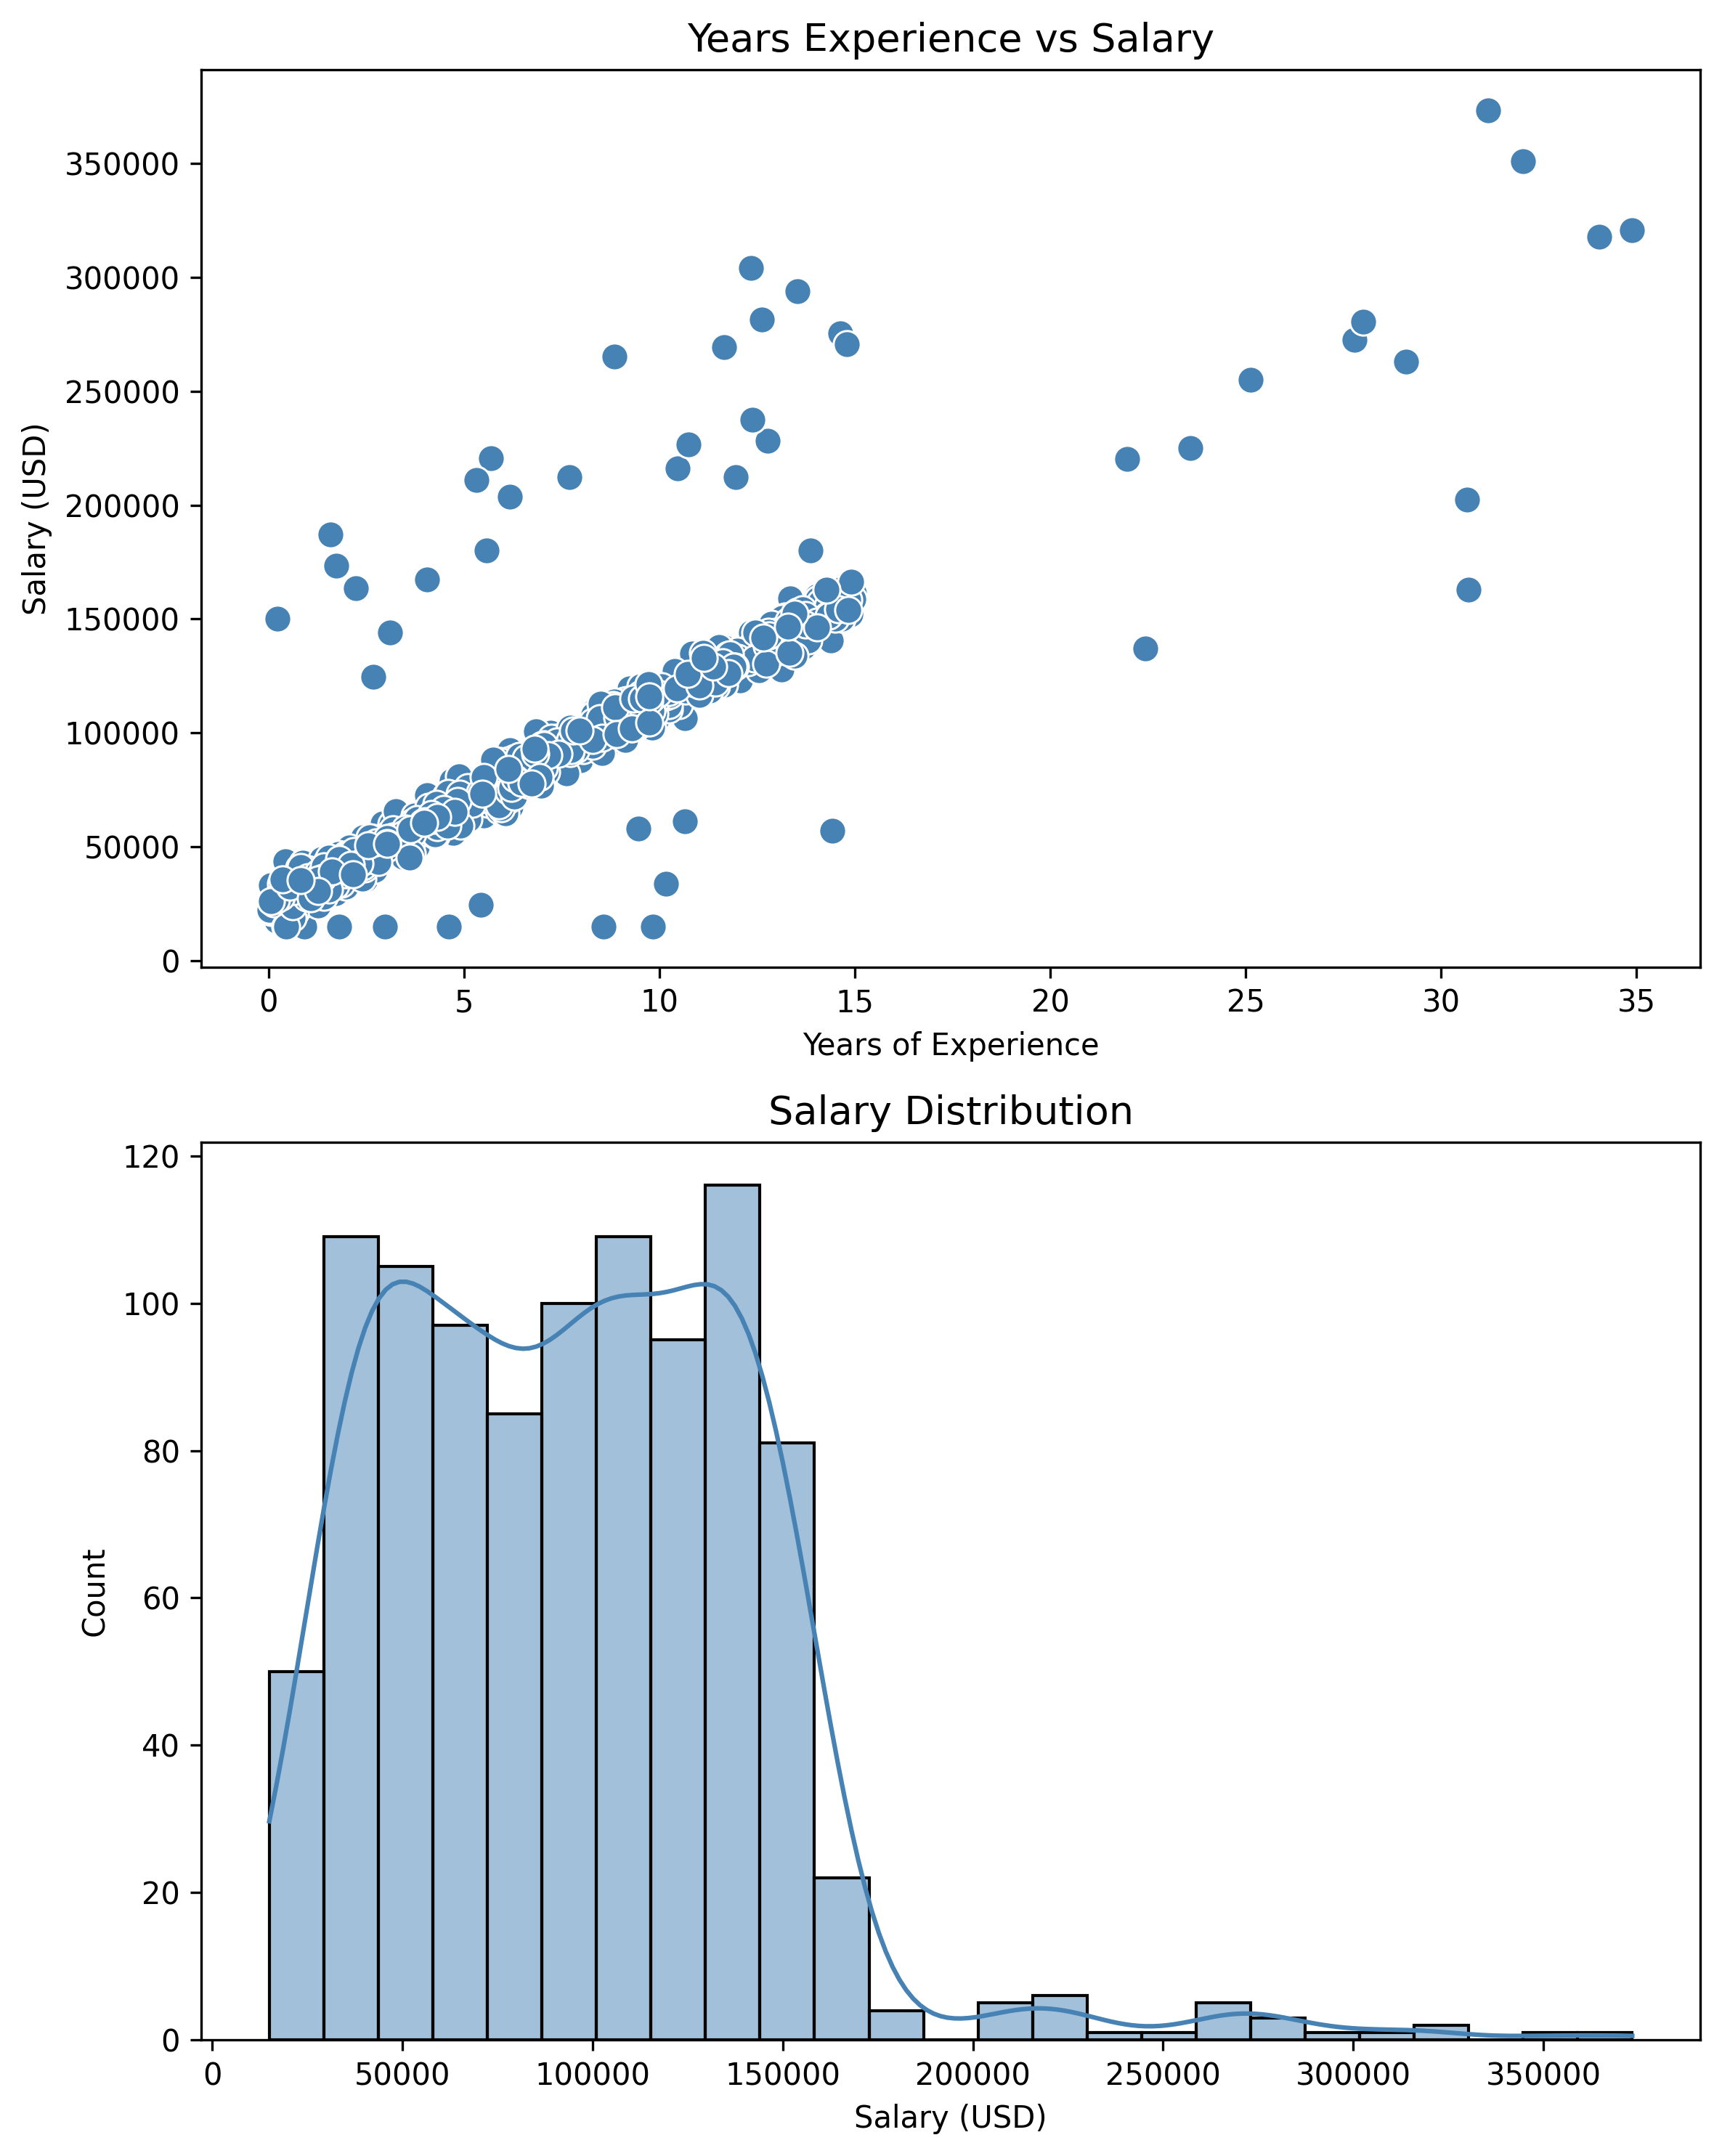
\includegraphics[width=\textwidth]{images/exploratory_analysis.png}
   	 \caption{Análisis exploratorio: dispersión y distribución del salario}
   	 \label{fig:exploratory}
	\end{figure}

\subsection{Superponer en el mismo gráfico las rectas obtenidas por ambos métodos.}

	\begin{figure}[h!]
    	\centering
    	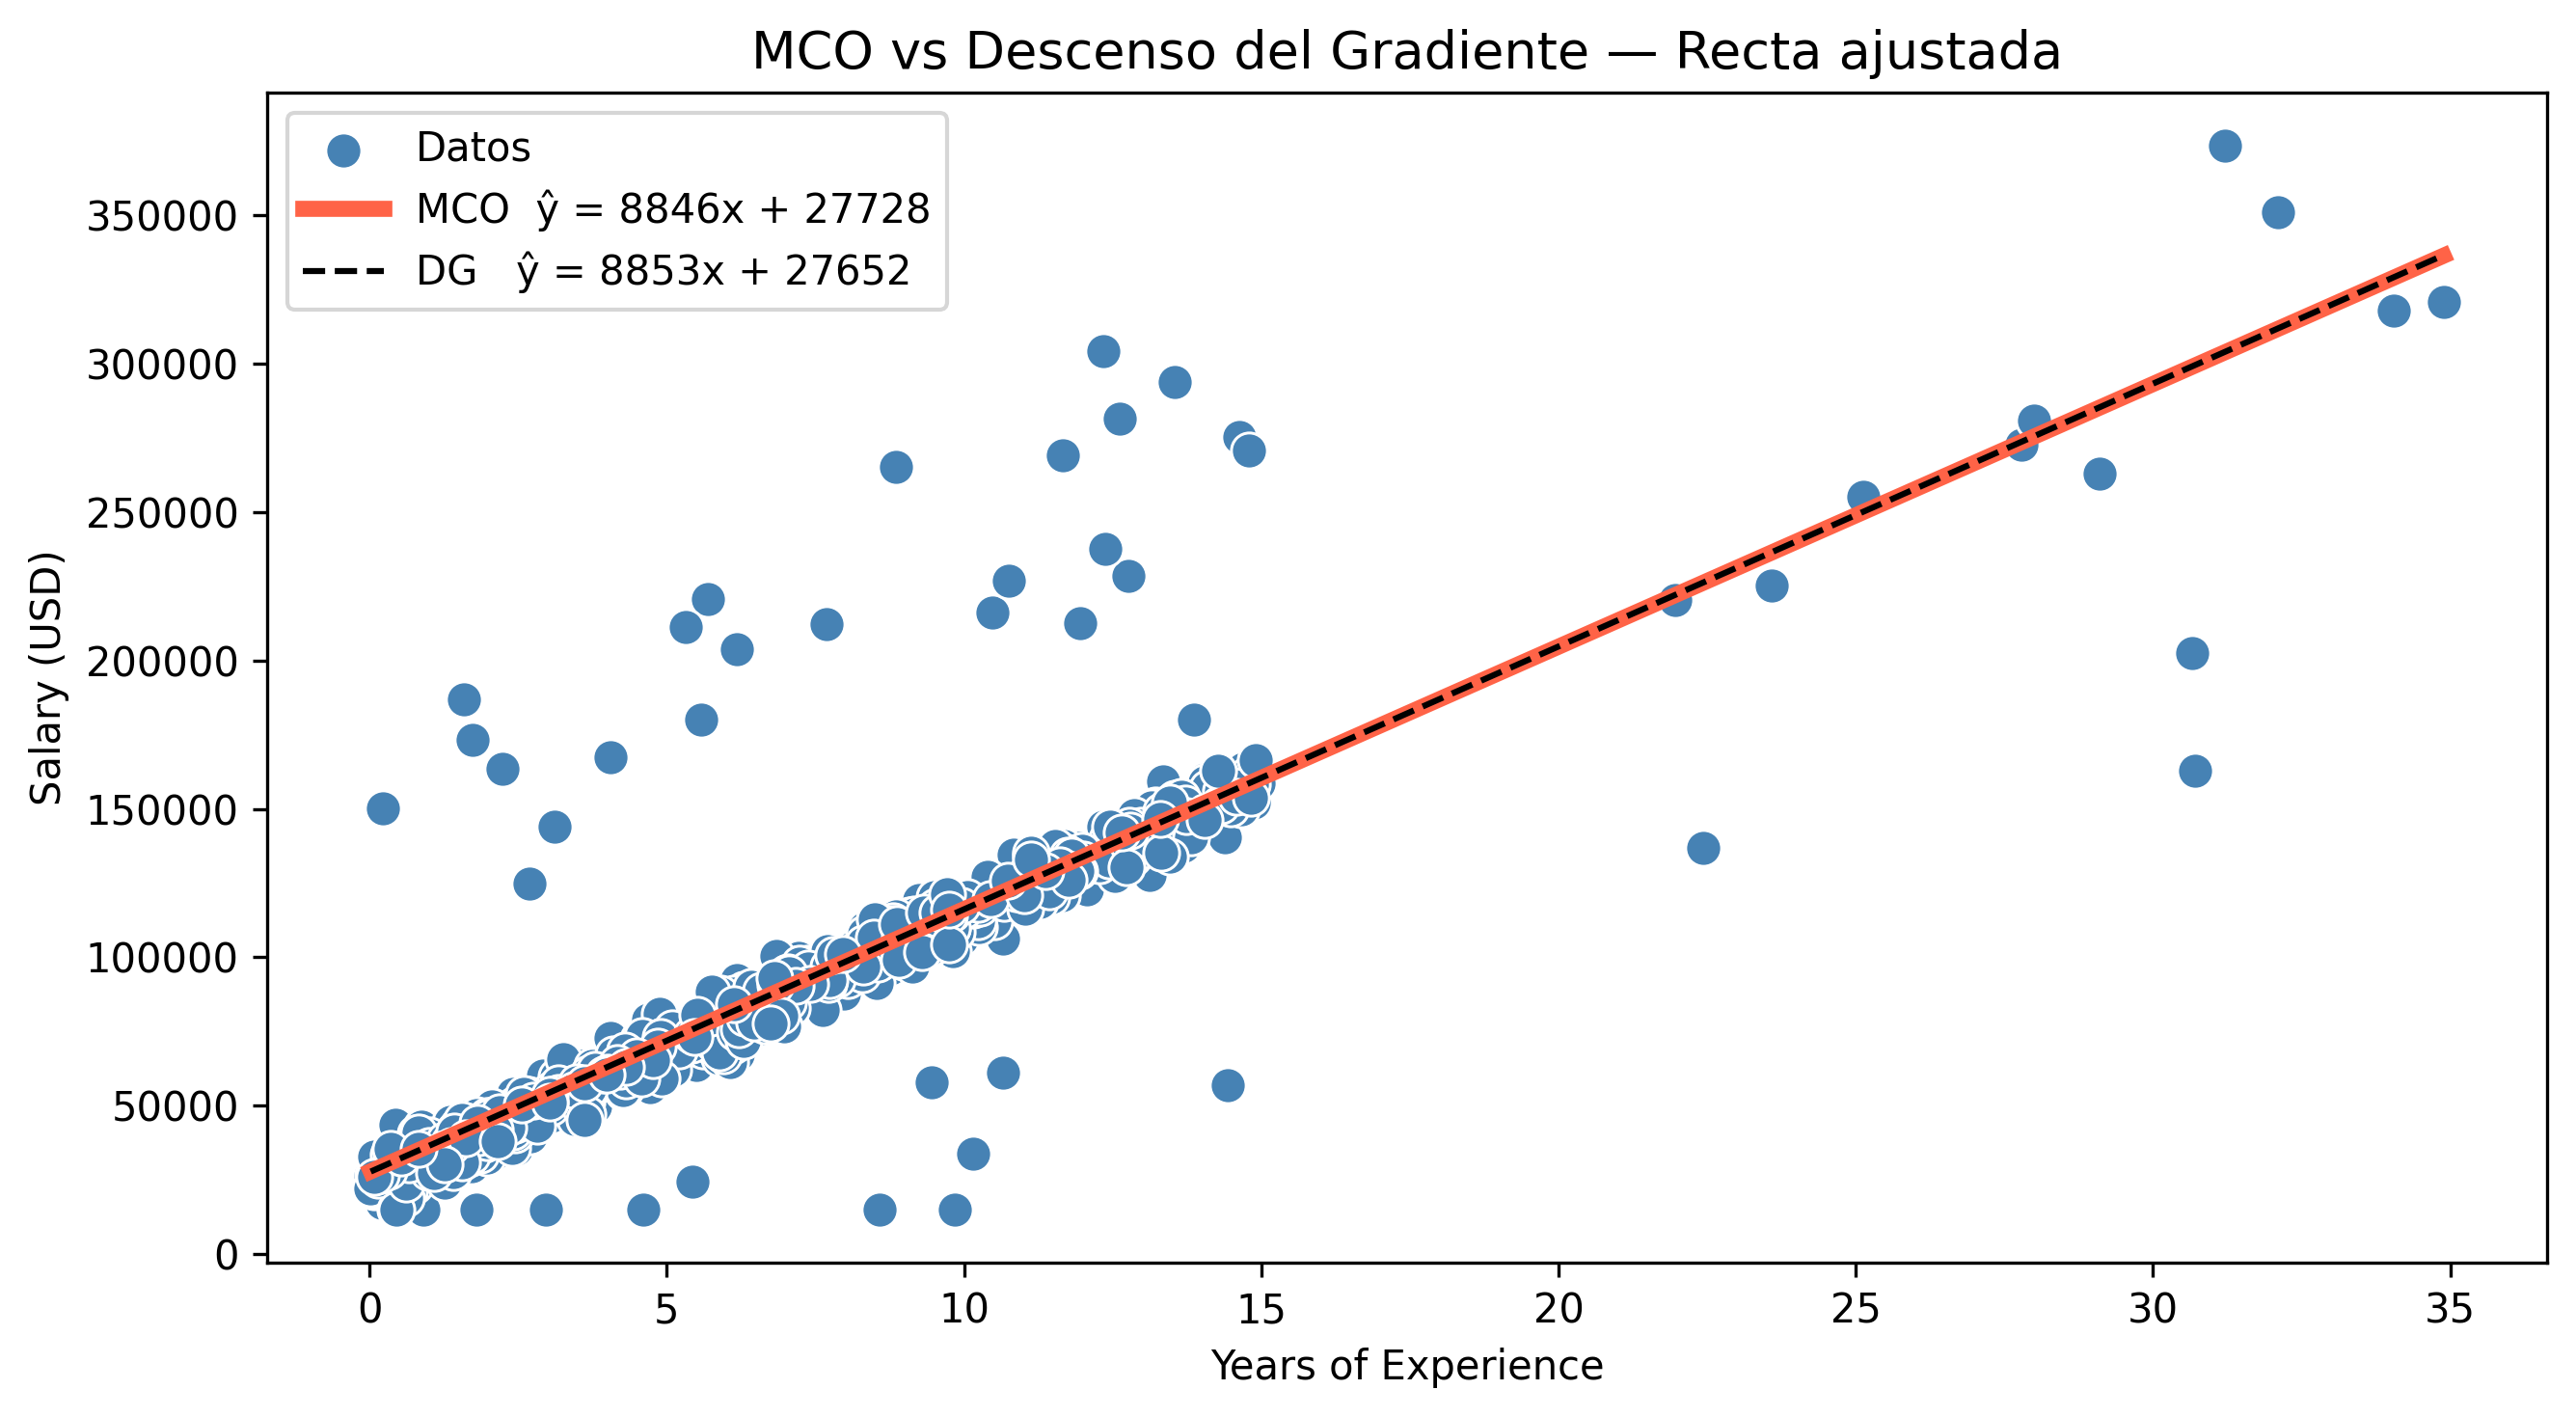
\includegraphics[width=\textwidth]{images/regresion_comparacion.png}
   	 \caption{Rectas ajustadas}
   	 \label{fig:exploratory}
	\end{figure}

\newpage
\subsection{Graficar la evolución de la función de pérdida durante las iteraciones del Descenso del Gradiente.}

	\begin{figure}[h!]
    	\centering
    	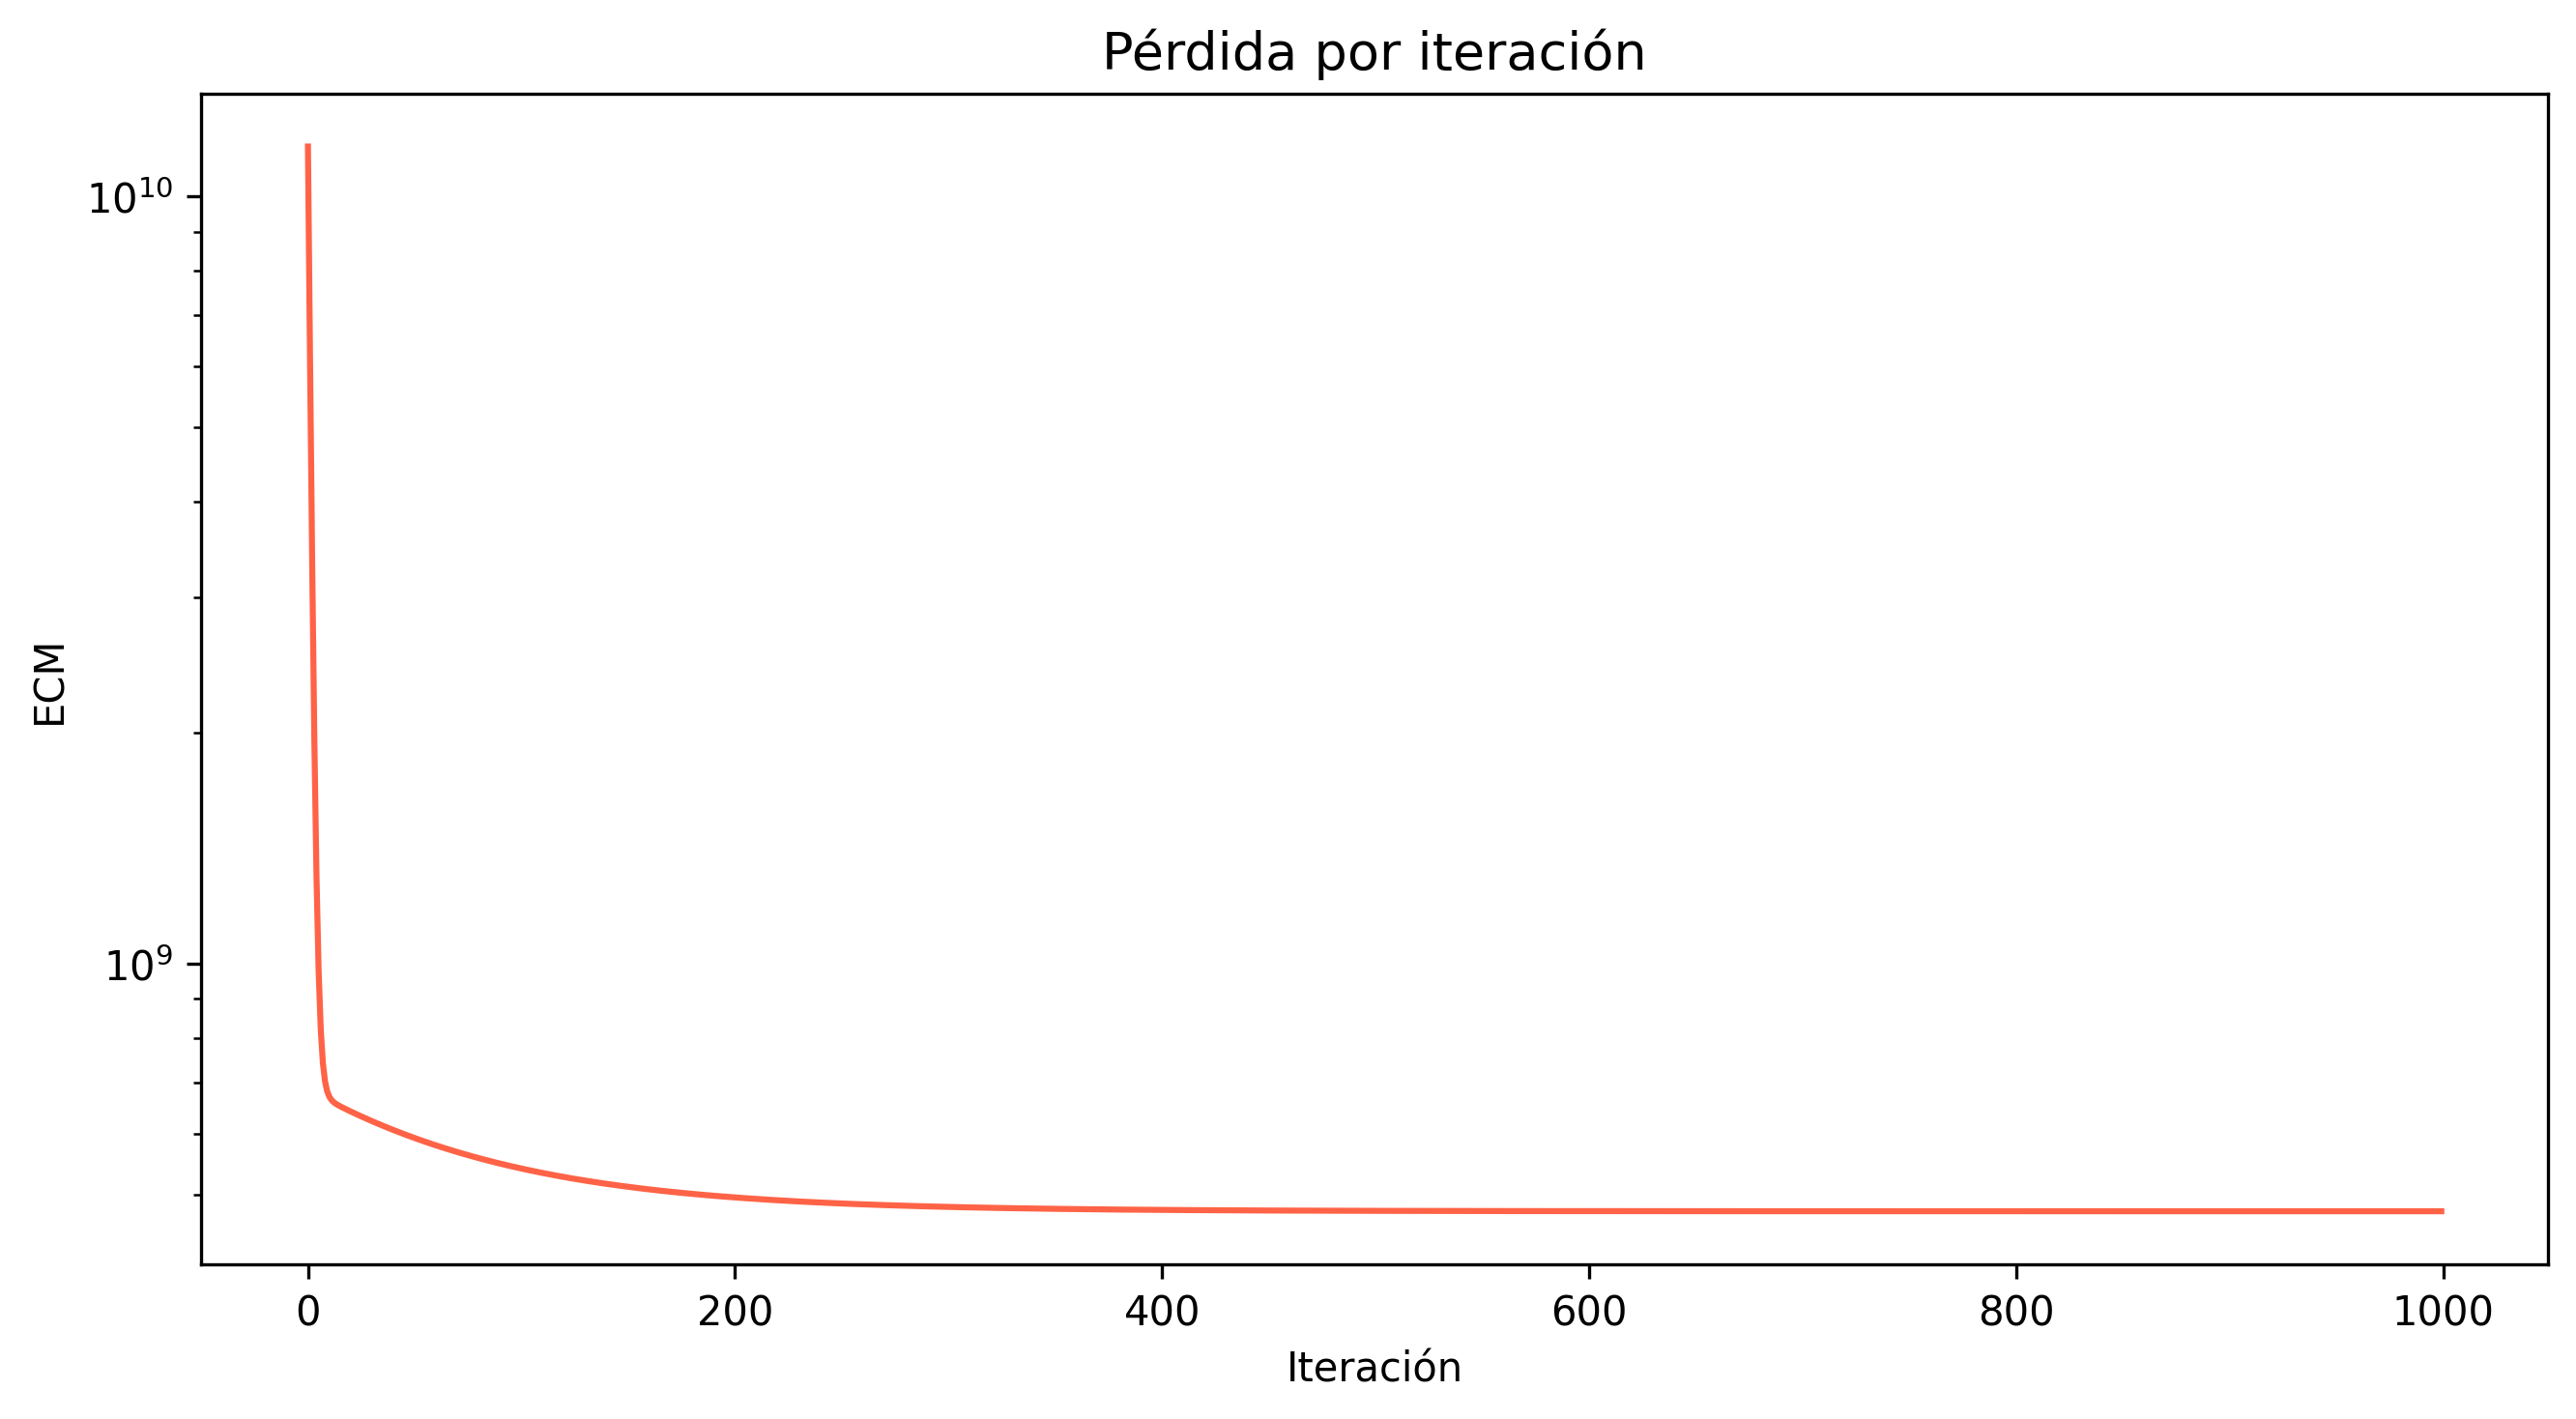
\includegraphics[width=\textwidth]{images/funcion_perdida.png}
   	 \caption{Función perdida}
   	 \label{fig:exploratory}
	\end{figure}
	
\newpage
\section{Segunda Parte: Análisis y Clasificación de la Calidad de la Leche mediante Regresión Logística}
\subsection{Preprocesamiento de Datos}

\begin{itemize}
    \item[$\scalebox{0.7}{$\blacksquare$}$] Carga y exploración inicial del dataset.
		
		\begin{table}[h!]
		\centering
		\caption{Información del Dataset}
		\begin{tabular}{clcc}
		\hline
		\textbf{\#} & \textbf{Columna} & \textbf{No. Nulos} & \textbf{Tipo} \\
		\hline
		0 & pH          & 1059 & \texttt{float64} \\
		1 & Temperature & 1059 & \texttt{int64}   \\
		2 & Taste       & 1059 & \texttt{int64}   \\
		3 & Odor        & 1059 & \texttt{int64}   \\
		4 & Fat         & 1059 & \texttt{int64}   \\
		5 & Turbidity   & 1059 & \texttt{int64}   \\
		6 & Colour      & 1059 & \texttt{int64}   \\
		7 & Grade       & 1059 & \texttt{str}     \\
		\hline
		\end{tabular}
		\end{table}

    \item[$\scalebox{0.7}{$\blacksquare$}$] Identificación y tratamiento de valores faltantes o atípicos.

	Las columnas Taste, Odor, Fat, turbidity solo tienen valores 1 y 0, pH, Temperature serán Escalados y Colour no se observan valors atipicos, no fue necesario tratamiento de valores atípicos

    \item[$\scalebox{0.7}{$\blacksquare$}$] Codificación de la variable objetivo.

	Se utilizó \texttt{LabelEncoder} de \texttt{scikit-learn}:
	para codificar la variable objetivo, con la siguiente codificación por clase:
	
	\begin{table}[h!]
	\centering
	\begin{tabular}{lc}
	\hline
	\textbf{Clase} & \textbf{Código} \\
	\hline
	\texttt{high}   & 0 \\
	\texttt{low}    & 1 \\
	\texttt{medium} & 2 \\
	\hline
	\end{tabular}
	\caption{Codificación de la variable objetivo \texttt{Grade}}
	\end{table}

    \item[$\scalebox{0.7}{$\blacksquare$}$] Escalado de características numéricas (pH y Temperatura).

	Se utilizó \texttt{StandardScaler} de \texttt{scikit-learn}:

	\begin{verbatim}
	from sklearn.preprocessing import StandardScaler
	\end{verbatim}
	
	para escalar las variables \texttt{pH} y \texttt{Temperature}, generando dos nuevas columnas para ser usadas en la regresión:
	
	\begin{verbatim}
	"pH_escalado", "Temprature_escalado"
	\end{verbatim}
\end{itemize}
	
\subsection{Análisis Estadístico Descriptivos}
\begin{itemize}
    \item[$\scalebox{0.7}{$\blacksquare$}$] Cálculo de estadísticas descriptivas:

    \begin{center}
       \resizebox{\textwidth}{!}{\begin{tabular}{lrrrrrrrrrrr}
\toprule
 & count & mean & std & min & 10\% & 25\% & 50\% & 75\% & 90\% & 95\% & max \\
\midrule
pH & 1059 & 6.6 & 1.4 & 3.0 & 4.5 & 6.5 & 6.7 & 6.8 & 8.6 & 9.0 & 9.5 \\
Temprature & 1059 & 44.2 & 10.1 & 34.0 & 36.0 & 38.0 & 41.0 & 45.0 & 55.0 & 66.0 & 90.0 \\
Taste & 1059 & 0.5 & 0.5 & 0.0 & 0.0 & 0.0 & 1.0 & 1.0 & 1.0 & 1.0 & 1.0 \\
Odor & 1059 & 0.4 & 0.5 & 0.0 & 0.0 & 0.0 & 0.0 & 1.0 & 1.0 & 1.0 & 1.0 \\
Fat  & 1059 & 0.7 & 0.5 & 0.0 & 0.0 & 0.0 & 1.0 & 1.0 & 1.0 & 1.0 & 1.0 \\
Turbidity & 1059 & 0.5 & 0.5 & 0.0 & 0.0 & 0.0 & 0.0 & 1.0 & 1.0 & 1.0 & 1.0 \\
Colour & 1059 & 251.8 & 4.3 & 240.0 & 245.0 & 250.0 & 255.0 & 255.0 & 255.0 & 255.0 & 255.0 \\
Grade\_encoded & 1059 & 1.1 & 0.8 & 0.0 & 0.0 & 1.0 & 1.0 & 2.0 & 2.0 & 2.0 & 2.0 \\
pH\_escalado & 1059 & 0.0 & 1.0 & -2.6 & -1.5 & -0.1 & 0.0 & 0.1 & 1.4 & 1.7 & 2.1 \\
Temprature\_escalado & 1059 & 0.0 & 1.0 & -1.0 & -0.8 & -0.6 & -0.3 & 0.1 & 1.1 & 2.2 & 4.5 \\
\bottomrule
\end{tabular}}
    \end{center}

    \item[$\scalebox{0.7}{$\blacksquare$}$] Visualización mediante histogramas y diagramas de caja.
    \begin{figure}[h!]
    \centering
    
\includegraphics[width=0.45\textwidth]{images/histogramas/pH.png}
    
\includegraphics[width=0.45\textwidth]{images/histogramas/Temprature.png}
    
\includegraphics[width=0.45\textwidth]{images/histogramas/Taste.png}
    
\includegraphics[width=0.45\textwidth]{images/histogramas/Odor.png}
    
\includegraphics[width=0.45\textwidth]{images/histogramas/Fat.png}
    
\includegraphics[width=0.45\textwidth]{images/histogramas/Turbidity.png}
    
\includegraphics[width=0.45\textwidth]{images/histogramas/Colour.png}
   
    \caption{Distribución de variables numéricas}
    \label{fig:histogramas}
    \end{figure}

    
    \begin{center}
    \begin{tabular}{cccccccc}
    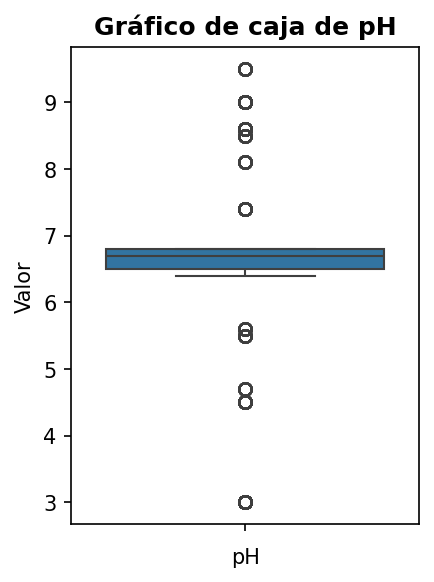
\includegraphics[width=0.18\textwidth]{images/cajas/pH.png} &
    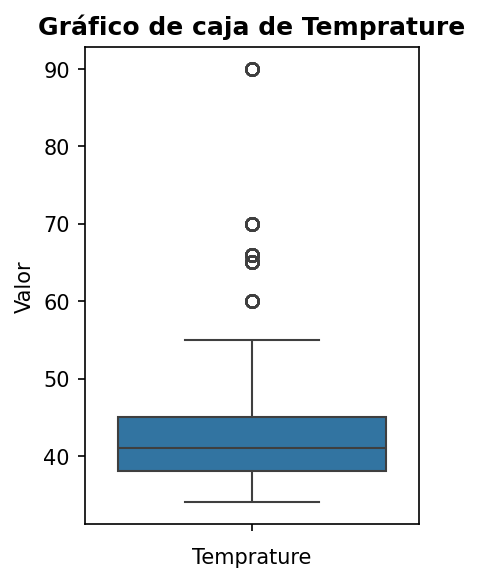
\includegraphics[width=0.18\textwidth]{images/cajas/Temprature.png} &
    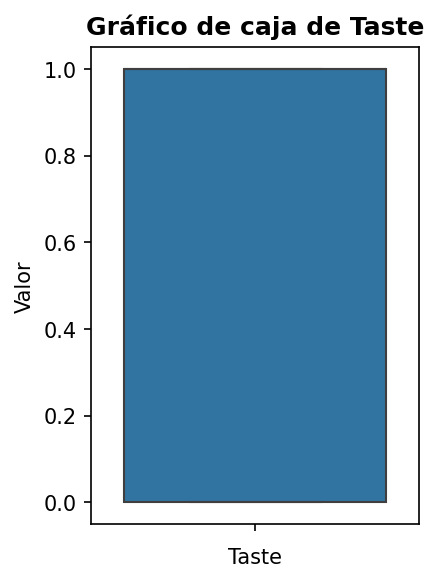
\includegraphics[width=0.18\textwidth]{images/cajas/Taste.png} &
    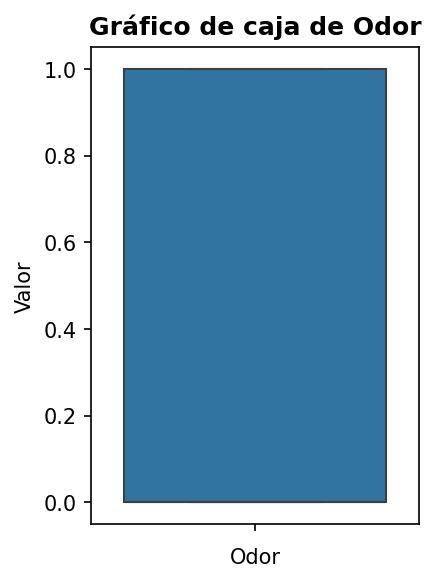
\includegraphics[width=0.18\textwidth]{images/cajas/Odor.png} \\
    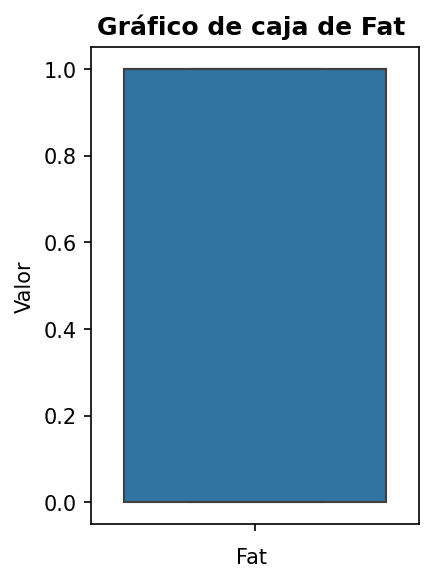
\includegraphics[width=0.18\textwidth]{images/cajas/Fat.png} &
    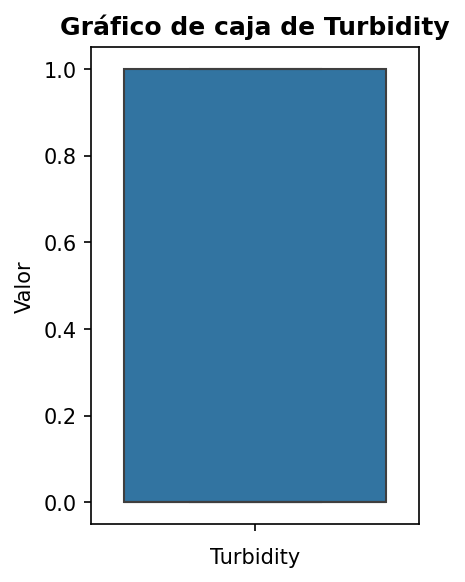
\includegraphics[width=0.18\textwidth]{images/cajas/Turbidity.png} &
    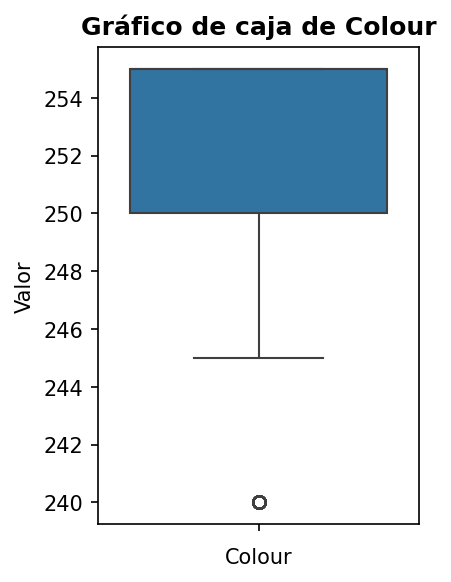
\includegraphics[width=0.18\textwidth]{images/cajas/Colour.png} 
    \end{tabular}
    \captionof{figure}{Gráfico de caja de variables numéricas}
    \label{fig:cajas}
     \end{center}
   
    

   
    \item[$\scalebox{0.7}{$\blacksquare$}$] Análisis de la distribución de la variable objetivo.
    \begin{center}
    \begin{tabular}{cccccccc}
    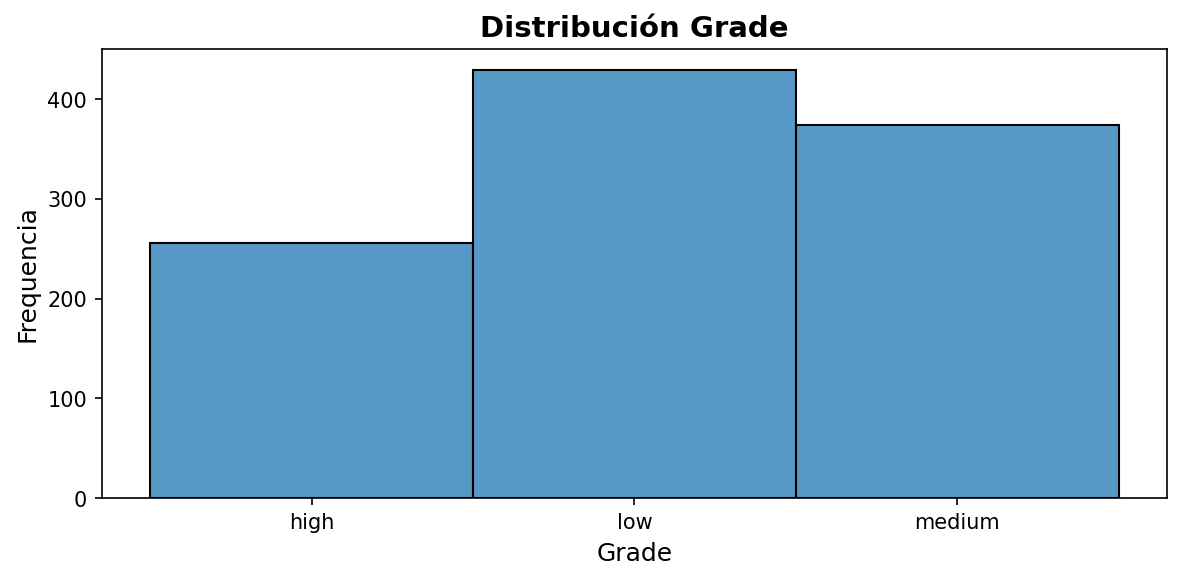
\includegraphics[width=0.64\textwidth]{images/histogramas/grade.png} &
    \end{tabular}
    \captionof{figure}{Distribución Variable Objetivo}
    \label{fig:Histograma}
     \end{center}
\end{itemize}

\subsection{Análisis de Correlación}
\begin{itemize}
	\item[$\scalebox{0.7}{$\blacksquare$}$] Cálculo de la matriz de correlación:
	
	\begin{center}
	    \resizebox{\linewidth}{!}{\begin{tabular}{lrrrrrrrrr}
\toprule
 & pH & Temprature & Taste & Odor & Fat  & Turbidity & Colour & pH\_escalado & Temprature\_escalado \\
\midrule
pH & 1.00 & 0.24 & -0.06 & -0.08 & -0.09 & 0.05 & -0.16 & 1.00 & 0.24 \\
Temprature & 0.24 & 1.00 & -0.11 & -0.05 & 0.02 & 0.19 & -0.01 & 0.24 & 1.00 \\
Taste & -0.06 & -0.11 & 1.00 & 0.02 & 0.32 & 0.06 & -0.08 & -0.06 & -0.11 \\
Odor & -0.08 & -0.05 & 0.02 & 1.00 & 0.31 & 0.46 & -0.04 & -0.08 & -0.05 \\
Fat  & -0.09 & 0.02 & 0.32 & 0.31 & 1.00 & 0.33 & 0.11 & -0.09 & 0.02 \\
Turbidity & 0.05 & 0.19 & 0.06 & 0.46 & 0.33 & 1.00 & 0.14 & 0.05 & 0.19 \\
Colour & -0.16 & -0.01 & -0.08 & -0.04 & 0.11 & 0.14 & 1.00 & -0.16 & -0.01 \\
pH\_escalado & 1.00 & 0.24 & -0.06 & -0.08 & -0.09 & 0.05 & -0.16 & 1.00 & 0.24 \\
Temprature\_escalado & 0.24 & 1.00 & -0.11 & -0.05 & 0.02 & 0.19 & -0.01 & 0.24 & 1.00 \\
\bottomrule
\end{tabular}}
	    \captionof{table}{Matriz de correlación de variables numéricas}
	    \label{tab:correlacion}
	\end{center}

	\item[$\scalebox{0.7}{$\blacksquare$}$] Visualización mediante mapa de calor:

	\begin{center}
	    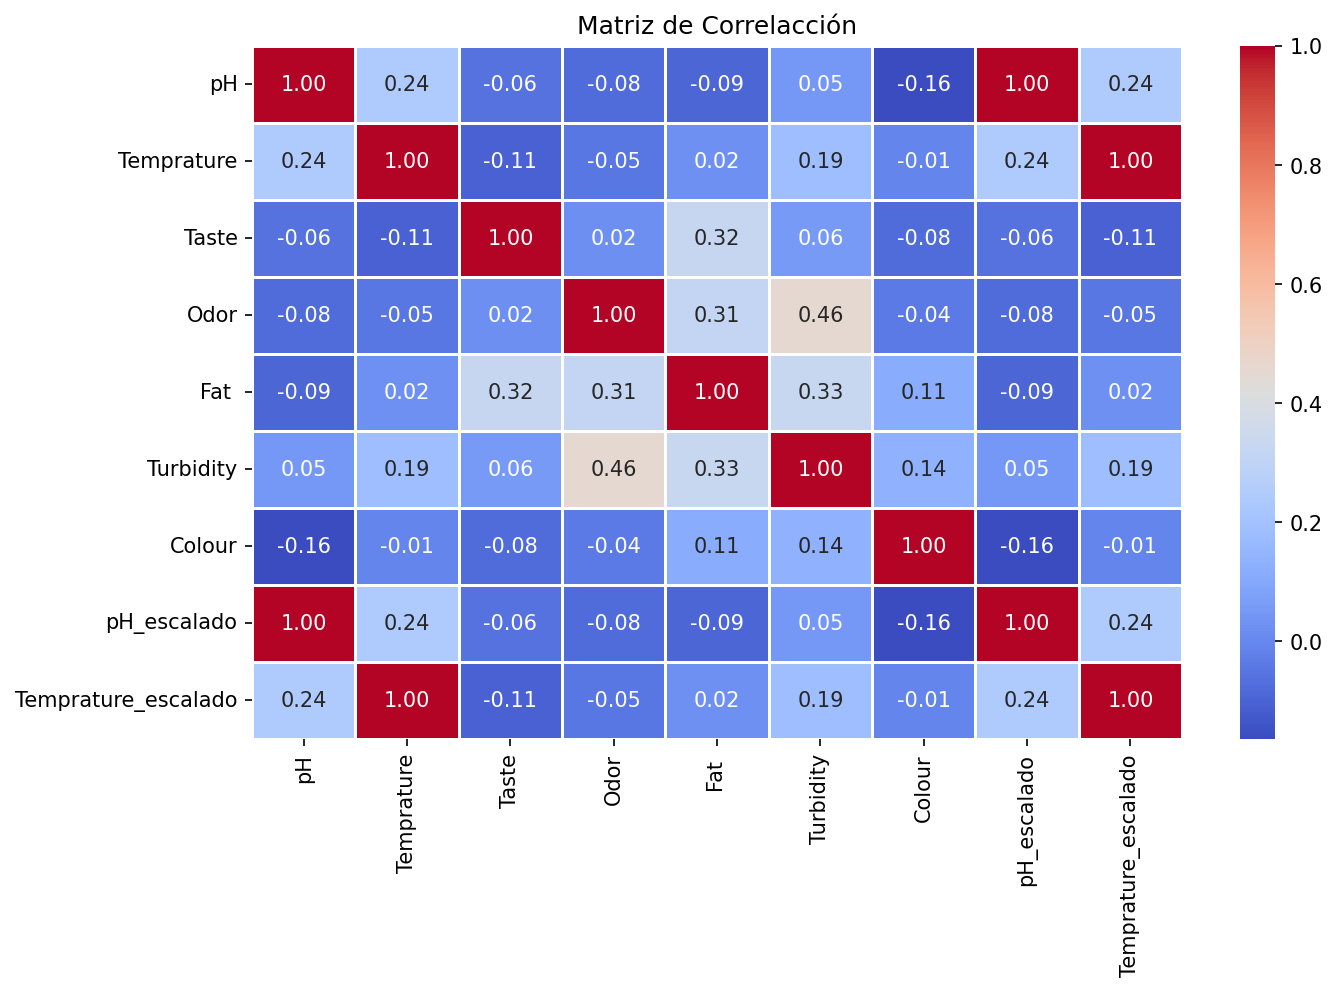
\includegraphics[width=0.8\textwidth]{images/correlacion.png}
	    \captionof{figure}{Mapa de calor}
	    \label{fig:matriz de correlacionl}
	\end{center}

	\item[$\scalebox{0.7}{$\blacksquare$}$] Interpretación de las relaciones entre variables:
\end{itemize}
	
	Lorem Ipsum is simply dummy text of the printing and typesetting industry. Lorem Ipsum has been the industry's standard dummy text ever since the 1500s, when an unknown printer took a galley of type and scrambled it to make a type specimen book. It has survived not only five centuries, but also the leap into electronic typesetting, remaining essentially unchanged. It was popularised in the 1960s with the release of Letraset sheets containing Lorem Ipsum passages, and more recently with desktop publishing software like Aldus PageMaker including versions of Lorem Ipsum.

\subsection{Implementación del Modelo de Regresión Logistica}

\begin{itemize}
	\item[$\scalebox{0.7}{$\blacksquare$}$] División del dataset en entrenamiento (80 \%) y prueba (20 \%).
	Se definieron las variables predictoras $X$ y la variable objetivo $y$:

	\begin{verbatim}
	X = df_milk[["Temprature_escalado", "pH_escalado", "Taste", 
	             "Odor", "Fat", "Turbidity", "Colour"]]
	y = df_milk["Grade_encoded"]
	\end{verbatim}
	
	El dataset fue dividido en conjuntos de entrenamiento y prueba con una proporción
	80/20 mediante \texttt{train\_test\_split} con \texttt{random\_state=42}:
	
	\begin{verbatim}
	X_train, X_test, y_train, y_test = train_test_split(X, y, 
	                                    test_size=0.2, random_state=42)
	\end{verbatim}

	\item[$\scalebox{0.7}{$\blacksquare$}$] Entrenamiento del modelo de regresión logística.

	Se entrenó un modelo de regresión logística con \texttt{max\_iter=1000}
	mediante \texttt{scikit-learn}:
	
	\begin{verbatim}
	model = LogisticRegression(max_iter=1000)
	model.fit(X_train, y_train)
	\end{verbatim}

	\item[$\scalebox{0.7}{$\blacksquare$}$] Evaluación del modelo utilizando
					\begin{itemize}
					
							\item[$\scalebox{0.3}{$\blacksquare$}$] Acurracy, Precision, Recall y F1 - score
									\begin{center}
									    \begin{tabular}{lr}
\toprule
 & Valor \\
Métrica &  \\
\midrule
Accuracy & 0.8066 \\
Precision & 0.8140 \\
Recall & 0.8066 \\
F1-Score & 0.8080 \\
\bottomrule
\end{tabular}
									    \captionof{table}{Métricas de evaluación del modelo de Regresión Logística}
									    \label{tab:metricas}
									\end{center}
							\item[$\scalebox{0.3}{$\blacksquare$}$] Matriz de confusión
									\begin{center}
									    \includegraphics[width=0.8\textwidth]{images/matriz\_confusion.png}
									    \captionof{figure}{Matriz de confusión}
									    \label{fig:matriz de confusion}
									\end{center}

					\end{itemize}
	\item[$\scalebox{0.7}{$\blacksquare$}$] Interpretación de los coeficientes del modelo
					\begin{center}
    						\resizebox{\linewidth}{!}{\begin{tabular}{lrrrrrrr}
\toprule
 & Temprature\_escalado & pH\_escalado & Taste & Odor & Fat\  & Turbidity & Colour \\
\midrule
high & -0.9688 & 0.2911 & 0.2944 & 1.9642 & 3.4452 & 0.0309 & 0.0829 \\
low & 2.6199 & -0.4237 & 1.7454 & -0.0962 & -0.9904 & 1.8004 & 0.2341 \\
medium & -1.6511 & 0.1326 & -2.0397 & -1.8681 & -2.4549 & -1.8313 & -0.3170 \\
\bottomrule
\end{tabular}}
    						\captionof{table}{Coeficientes del modelo de Regresión Logística}
    						\label{tab:coeficientes}
					\end{center}
					
					% Clase Alta
							\subsubsection*{Clase: Alta (Buena)}
							\begin{center}
							\begin{tabular}{lcp{8cm}}
							\hline
							\textbf{Característica} & \textbf{Coeficiente} & \textbf{Interpretación} \\
							\hline
							Fat         & $+3.45$ & \textbf{Característica más importante} — la categoría codificada como 1 está fuertemente asociada con la alta calidad en la leche \\
							Odor        & $+1.96$ & la categoría codificada como 1 está fuertemente asociada con la alta calidad en la leche \\
							Taste       & $+0.29$ & la categoría codificada como 1 tiene un nexo débil con la alta calidad en la leche \\
							pH          & $+0.29$ & un pH alto puede tener un leve impacto positivo en la calidad de la leche \\
							Turbidity   & $+0.03$ & la categoría codificada como 1 tiene un efecto prácticamente nulo en la alta calidad de la leche \\
							Colour      & $+0.08$ & el color puede no tener impacto en la calidad de la leche \\
							Temperature & $\mathbf{-0.97}$ & una temperatura alta puede tener un impacto negativo en la calidad de la leche \\
							\hline
							\end{tabular}
							\end{center}
							
							% Clase Baja
							\subsubsection*{Clase: Baja (Mala)}
							\begin{center}
							\begin{tabular}{lcp{8cm}}
							\hline
							\textbf{Característica} & \textbf{Coeficiente} & \textbf{Interpretación} \\
							\hline
							Temperature & $\mathbf{+2.62}$ & \textbf{Característica importante} — altas temperaturas indican una mala calidad en la leche \\
							Turbidity   & $+1.80$ & la categoría codificada como 1 está fuertemente asociada con la mala calidad en la leche \\
							Taste       & $+1.75$ & la categoría codificada como 1 está fuertemente asociada con la mala calidad en la leche \\
							Odor        & $-0.10$ & efecto prácticamente nulo \\
							Fat         & $-0.99$ & la categoría codificada como 1 está fuertemente asociada con poca probabilidad de mala calidad en la leche \\
							Colour      & $+0.23$ & un fuerte color puede tener un impacto leve en la mala calidad de la leche \\
							pH          & $-0.42$ & un pH bajo puede estar levemente asociado a la mala calidad en la leche \\
							\hline
							\end{tabular}
							\end{center}
							
							% Clase Media
							\subsubsection*{Clase: Media (Moderada)}
							\begin{center}
							\begin{tabular}{lcp{8cm}}
							\hline
							\textbf{Característica} & \textbf{Coeficiente} & \textbf{Interpretación} \\
							\hline
							Taste       & $\mathbf{-2.04}$ & la categoría codificada como 1 está fuertemente asociada en la baja probabilidad de calidad media en la leche \\
							Fat         & $\mathbf{-2.45}$ & la categoría codificada como 1 está fuertemente asociada en la baja probabilidad de calidad media en la leche \\
							Odor        & $\mathbf{-1.87}$ & la categoría codificada como 1 está fuertemente asociada en la baja probabilidad de calidad media en la leche \\
							Turbidity   & $\mathbf{-1.83}$ & la categoría codificada como 1 está fuertemente asociada en la baja probabilidad de calidad media en la leche \\
							Temperature & $-1.65$ & la alta temperatura tiene un impacto negativo en la probabilidad de calidad media en la leche \\
							Colour      & $-0.32$ & el color fuerte puede tener un impacto leve en la baja probabilidad de calidad media en la leche \\
							pH          & $+0.13$ & el pH puede no tener impacto en la probabilidad de calidad media en la leche \\
							\hline
							\end{tabular}
							\end{center}
							
							% Resumen
							\subsubsection*{Resumen}
							\begin{itemize}
							    \item[$\scalebox{0.7}{$\blacksquare$}$] \textbf{Fat y Odor} son las características principales para identificar leche de buena calidad.
							    \item[$\scalebox{0.7}{$\blacksquare$}$] \textbf{Temperature y Turbidity} son las señales más fuertes de mala calidad en la leche — temperatura tibia y categoría 1 en la turbidez.
							    \item[$\scalebox{0.7}{$\blacksquare$}$] \textbf{Calidad media} está constantemente vinculada a la ausencia del valor 1 en las categorías Taste, Fat, Odor y Turbidity.
							\end{itemize}

	\item[$\scalebox{0.7}{$\blacksquare$}$] Discusión de resultados y posibles mejoras

	Lorem Ipsum is simply dummy text of the printing and typesetting industry. Lorem Ipsum has been the industry's standard dummy text ever since the 1500s, when an unknown printer took a galley of type and scrambled it to make a type specimen book. It has survived not only five centuries, but also the leap into electronic typesetting, remaining essentially unchanged. It was popularised in the 1960s with the release of Letraset sheets containing Lorem Ipsum passages, and more recently with desktop publishing software like Aldus PageMaker including versions of Lorem Ipsum.
\end{itemize}



\end{document}